%%%%%%%%%%%%%%%%%%%%%%%%%%%%%%%%%%%%%%%%%
% Intermediate report
% Version 1.0 (10/16/13)
%
% This template has been downloaded from:
% http://www.LaTeXTemplates.com
%
% Original Authors:
% Darren Chu
% Todd Detweiler
% Cody Kagawa
% Lauren Swanson
% Dogni Wang
%
%%%%%%%%%%%%%%%%%%%%%%%%%%%%%%%%%%%%%%%%%

%----------------------------------------------------------------------------------------
%	PACKAGES AND OTHER DOCUMENT CONFIGURATIONS
%----------------------------------------------------------------------------------------

\documentclass[a4paper, 11pt]{article} % Font size (can be 10pt, 11pt or 12pt) and paper size (remove a4paper for US letter paper)

\usepackage[protrusion=true,expansion=true]{microtype} % Better typography
\usepackage{graphicx} % Required for including pictures
\usepackage{wrapfig} % Allows in-line images
\usepackage{pdfpages}

\usepackage{mathpazo} % Use the Palatino font
\usepackage[T1]{fontenc} % Required for accented characters
\linespread{1.05} % Change line spacing here, Palatino benefits from a slight increase by default

\DeclareGraphicsExtensions{.pdf,.png,.jpg}


\makeatletter
\renewcommand\@biblabel[1]{\textbf{#1.}} % Change the square brackets for each bibliography item from '[1]' to '1.'
\renewcommand{\@listI}{\itemsep=0pt} % Reduce the space between items in the itemize and enumerate environments and the bibliography

\renewcommand{\maketitle}{ % Customize the title - do not edit title and author name here, see the TITLE block below
\begin{flushright} % Right align
{\LARGE\@title} % Increase the font size of the title

\vspace{50pt} % Some vertical space between the title and author name

{\large\@author} % Author name
\\\@date % Date

\vspace{40pt} % Some vertical space between the author block and abstract
\end{flushright}
}

%----------------------------------------------------------------------------------------
%	TITLE
%----------------------------------------------------------------------------------------

\title{\textbf{Intermediate Report for Object Creator Team}} 

\author{\textsc{Darren Chu\\Todd Detweiler\\Cody Kagawa\\Lauren Swanson\\Dogni Wang} % Author
\\{\textit{University of Puget Sound}}} % Institution

\date{\today} % Date

%----------------------------------------------------------------------------------------

\begin{document}

\maketitle % Print the title section

%----------------------------------------------------------------------------------------
%	ESSAY BODY
%----------------------------------------------------------------------------------------

\section*{Design Specification}

Our module will have four major components including a way to create an image, edit an image, save image, and a way to export the object as a JSON object. The Image Creation class will include functions to draw on a canvas, import an image, or use primitive shapes to construct each individual object. Image Creation will require a canvas, which will be provided by the Javascript Library. The canvas will report the coordinates of the object features, as to facilitate conversion into a .png format. Next, the Image Editing class will allow the user to manipulate the size and color of the object, while also providing access to an undo button. The functions of the Image Editing class will be accessible to the user through a toolbar type user interface. Thirdly, there will be a Save Image class which allows users to save pieces of their full object as as .png files. And finally, Export Object will be a class which is called upon exiting the canvas and will send the group of saved pieces to the Sharing Framework as a JSON object.

This Image Creation window, along side our canvas window, will prompt begin drawing part.” This prompt will acknowledge that the user is drawing a part of the character, which will be saved as a unique object. The user will be responsible for designating a name for the object, such as head.png, in order to be uniquely recognized for use in other modules. If the user chooses to draw their object, they will do so by drawing, naming, and saving each part individually. The Save Image class will save each piece as a .png file in a position in an array. When the user is finished saving each piece of their object, they will exit out of the Object creation window. This act of exiting will also call our Export Object class which will export the array of saved.png images to the Sharing Framework as a JSON object. Once on the sharing framework, the object and its pieces can be accessed and manipulated by other modules. Below, a full UML class diagram of these three major components and their functions are shown.

%------------------------------------------------

\section*{Design Rationale}

To create our model, we will be implementing an Abstract Factory software design pattern. Since an abstract factory is a group of factories that have a common theme this seems to fit the best. We have different classes that create objects and shapes in different ways (i.e. drawing, importing, geometric shapes) but all share the common theme of creating an image and eventually forming the object. These different forms of creation make up our different factories for image creation. All classes such as image creation, object creation, and editing have to do with images and JSON objects but handle them differently falling under our abstract factory model.

%------------------------------------------------

\section*{Design Architecture UML Diagram}
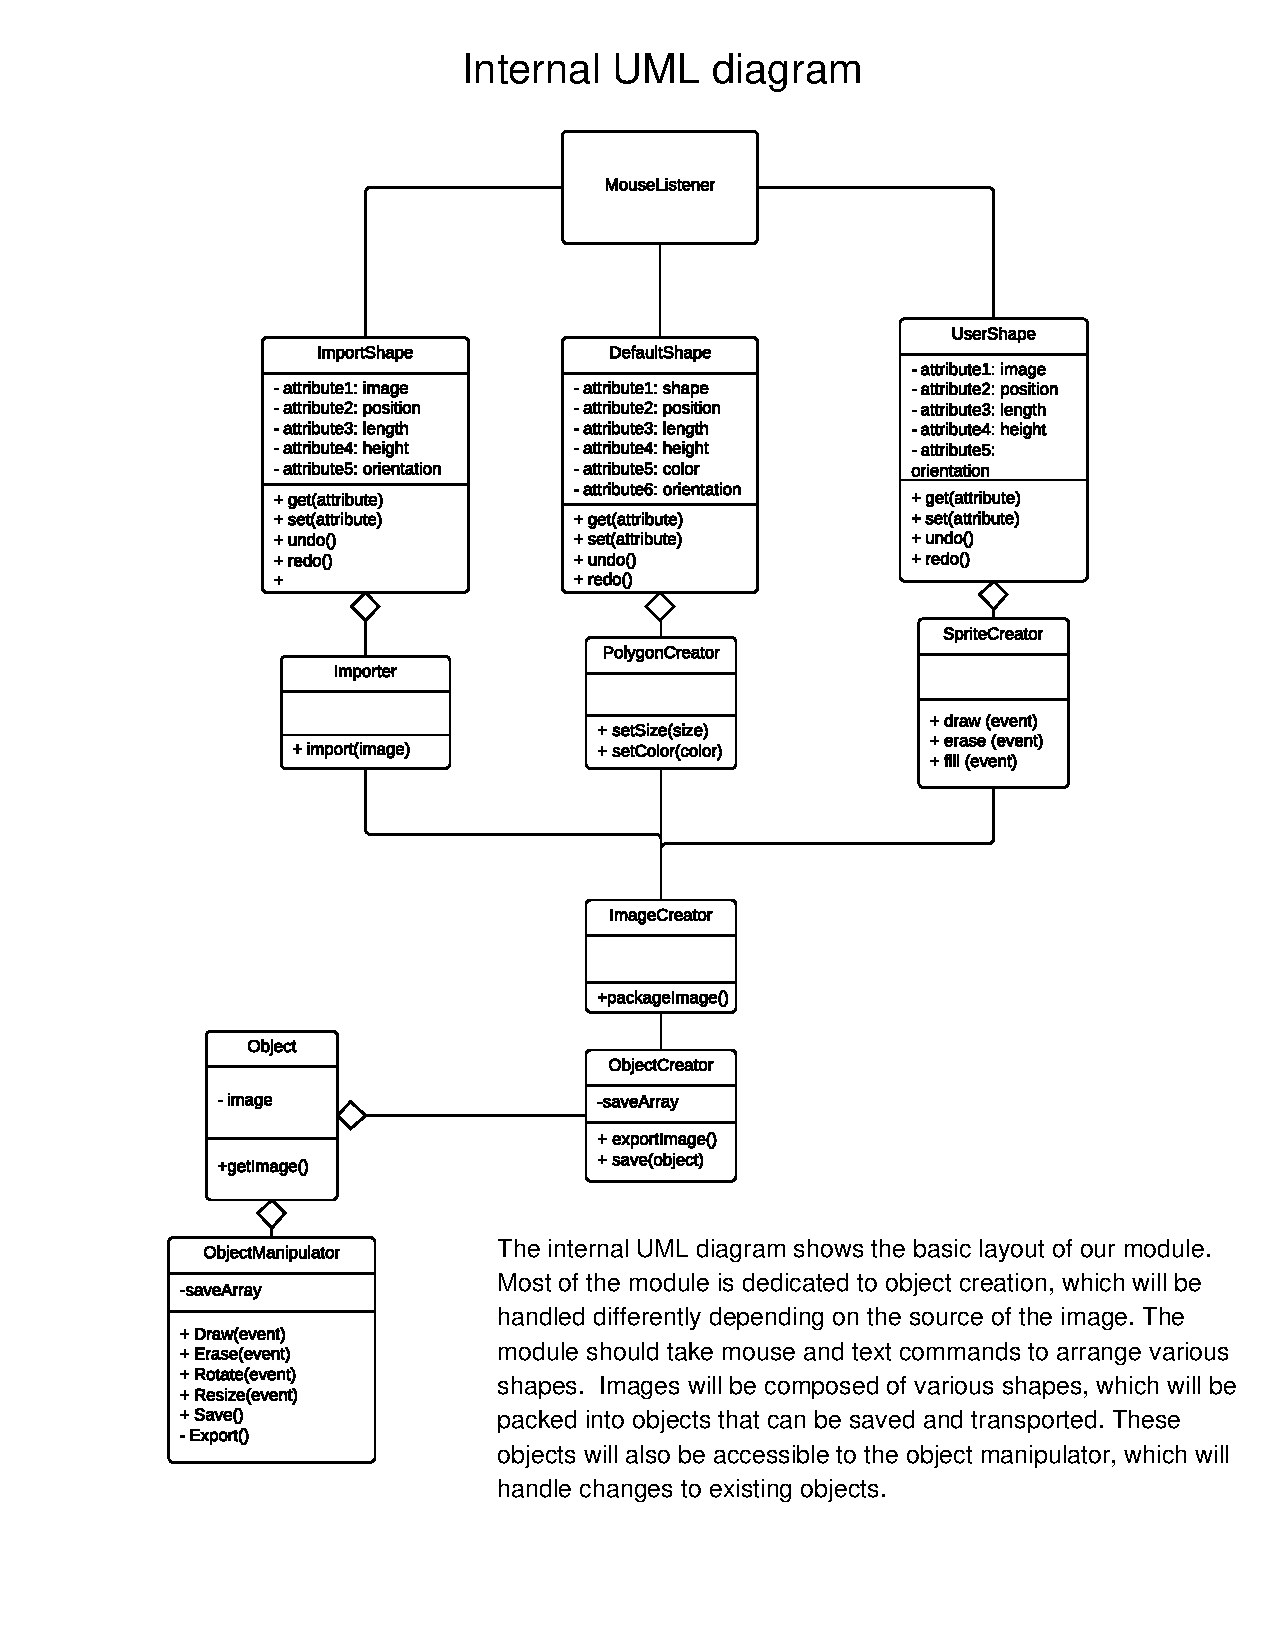
\includepdf[pages={1}]{ClassDiagramObjectModule1.pdf}
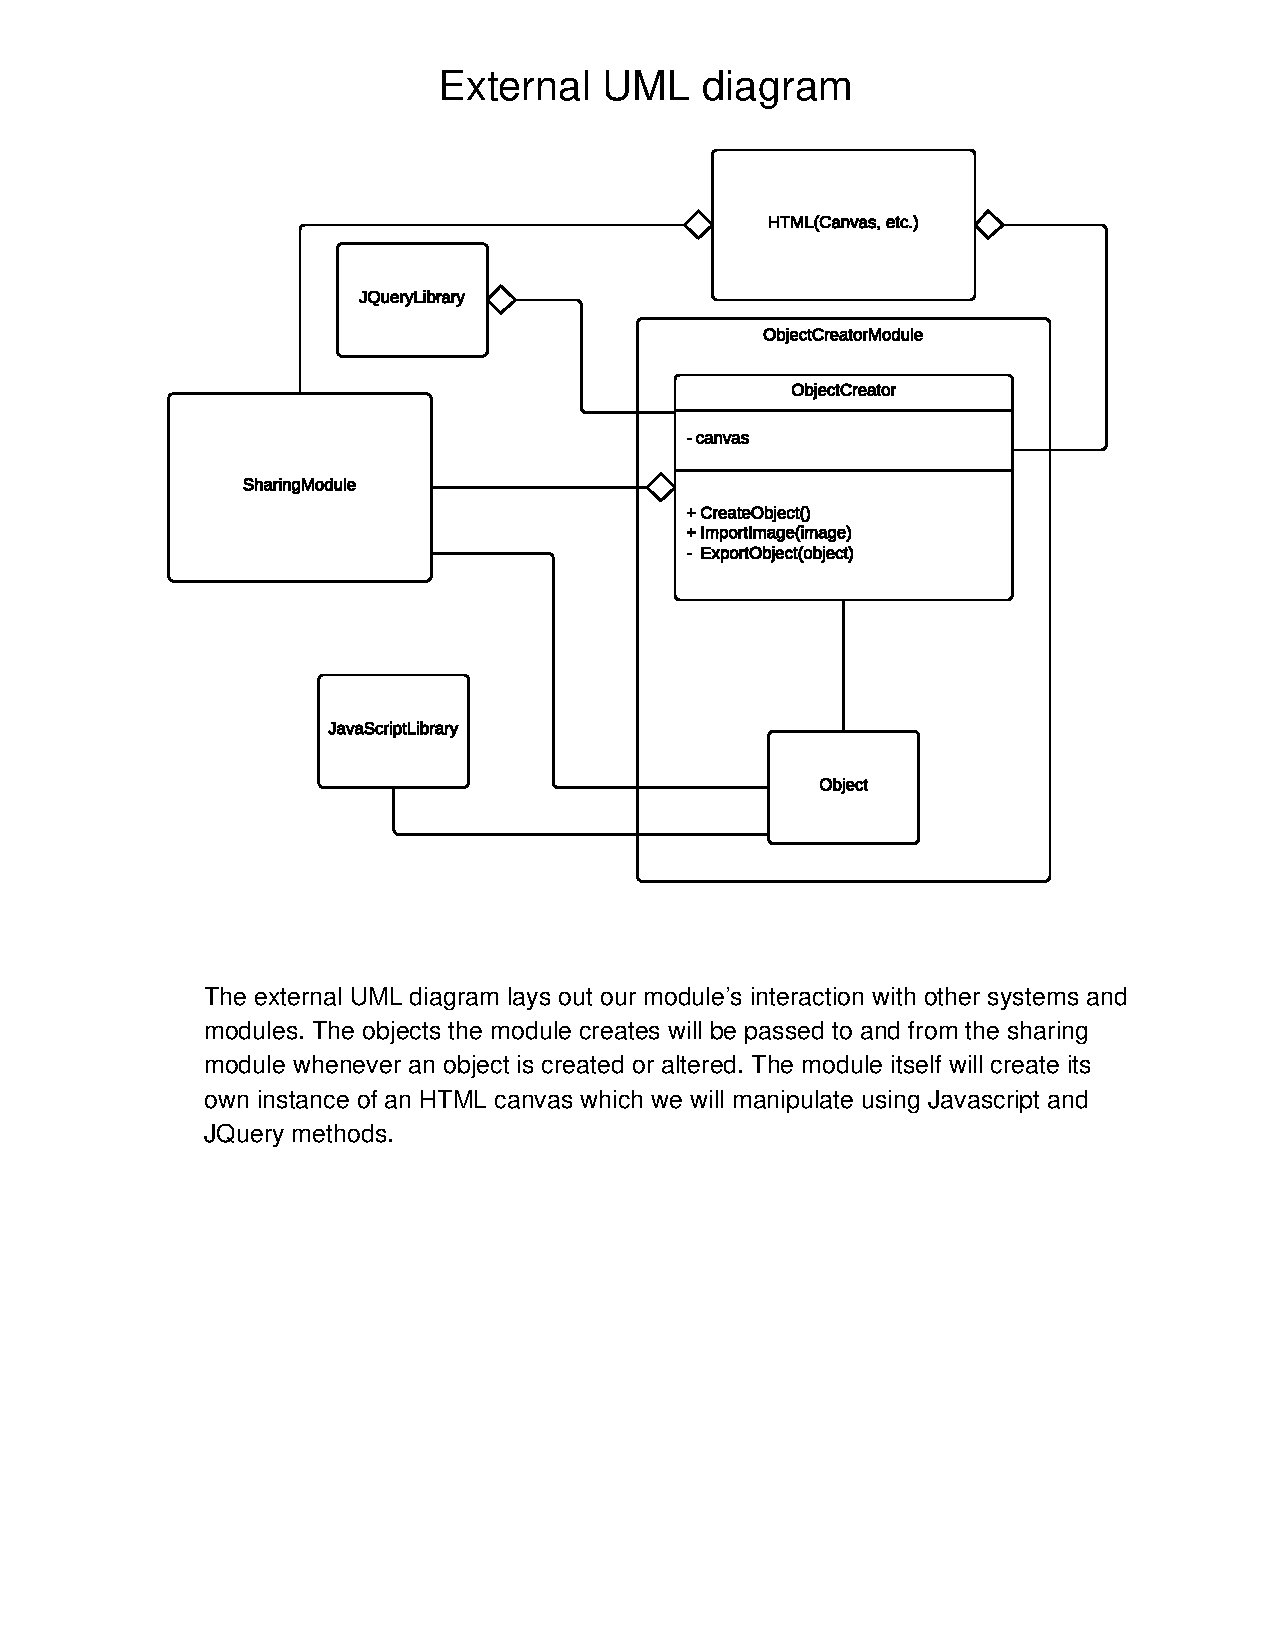
\includepdf[pages={1}]{ExternalFlowChart1.pdf}

%------------------------------------------------

\section*{Project Status}

The current state of our module is at the end of the design and planning phase. We have determined the structure of our module and how the user will interact with our functions. We have also determined how our module will interact with other modules of the application. We have established that our module will be exporting JSON array objects filled with .png files to the Sharing Framework. Before our first implementation stage, we will create four different functions. The following team members will be responsible for their listed implementations. Todd will be responsible for a general layout of our canvas, Cody for a free drawing function, Lauren for a saving and exporting function, and Dongni and Darren for the geometric drawing function. All members will collaborate on each part and provide assistance where needed. The timeline of our completion and implementation checkpoints can be seen on the Gantt timeline below.

%------------------------------------------------

\section*{Project Timeline}

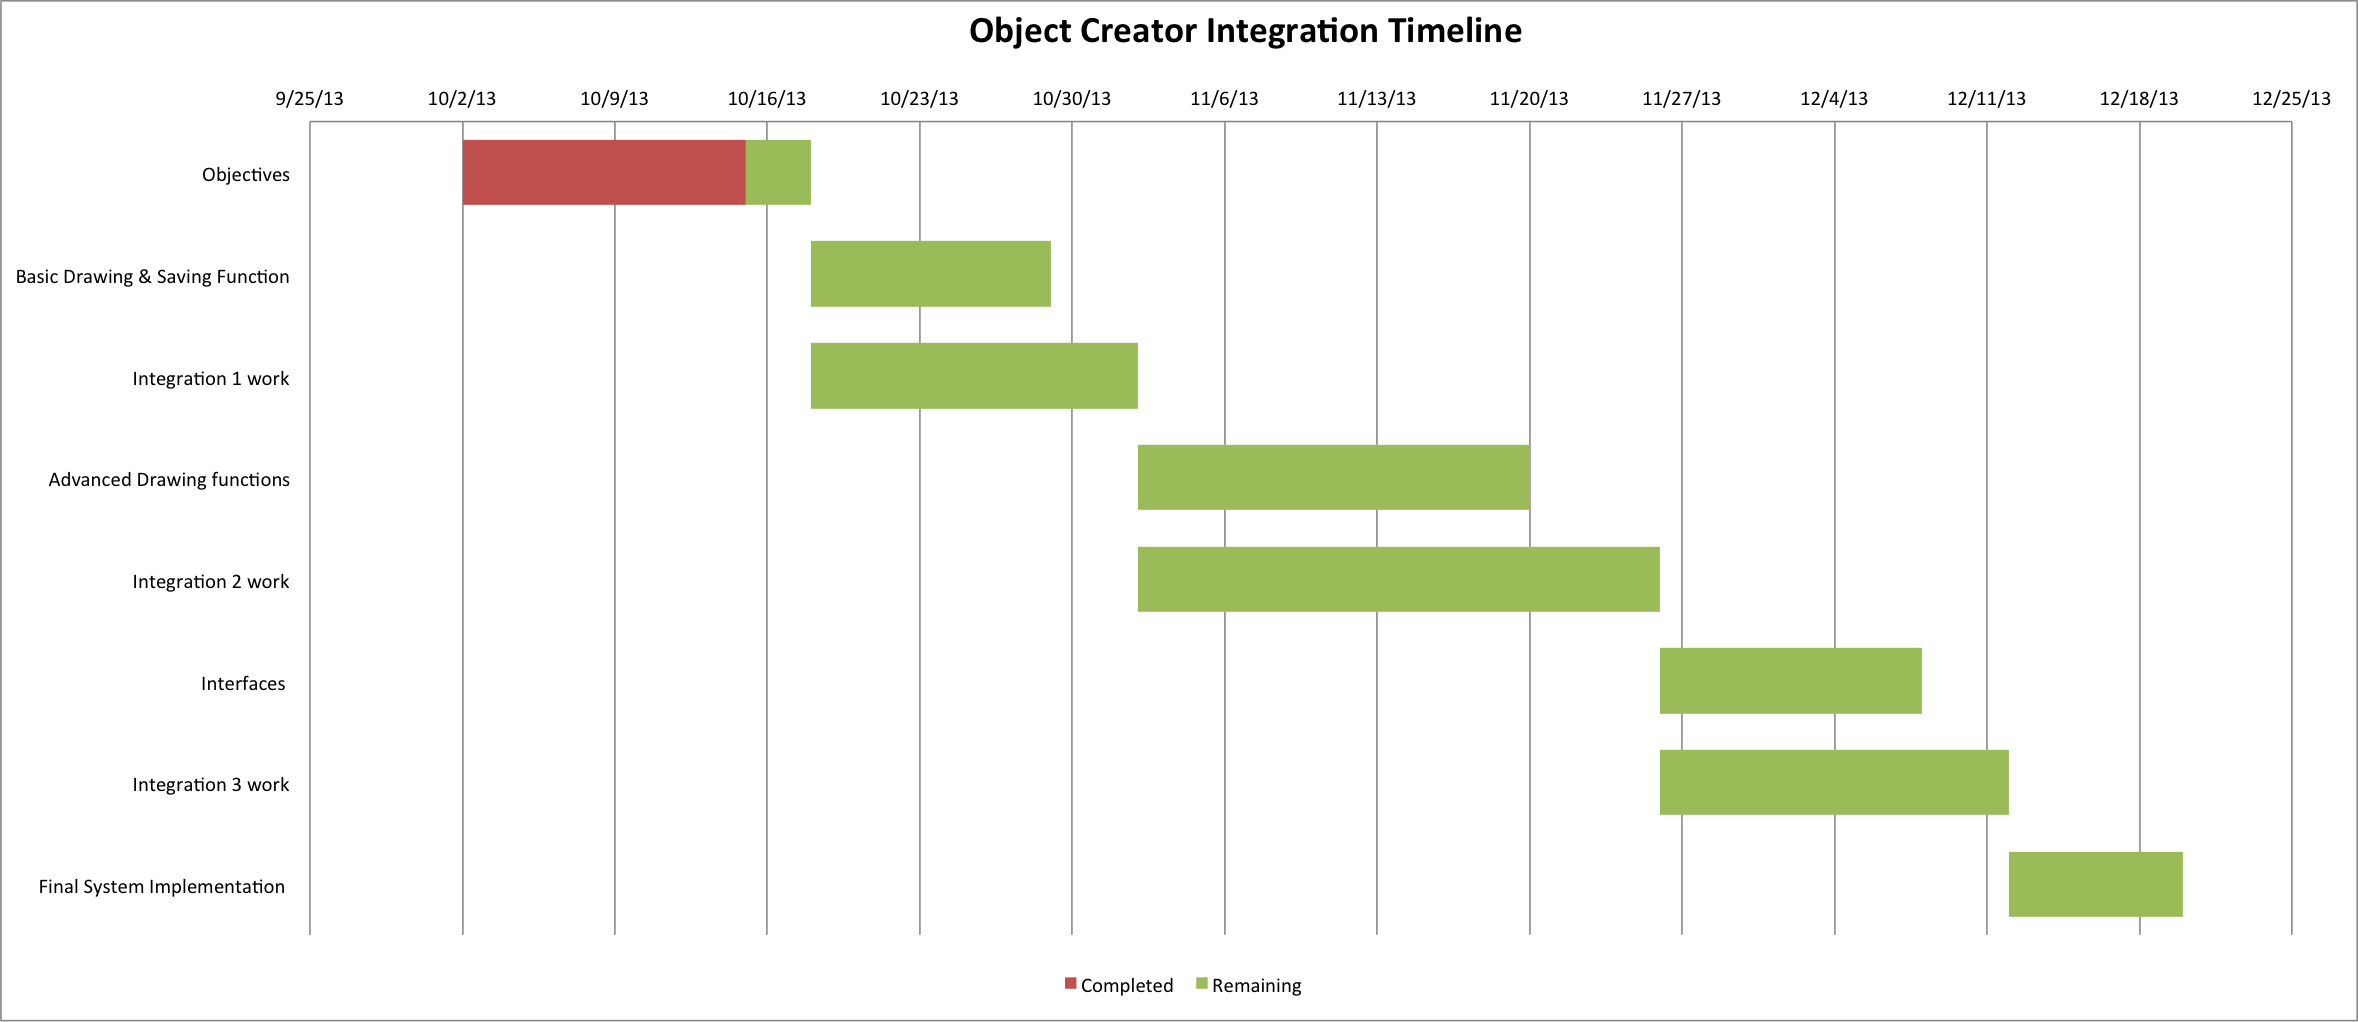
\includegraphics[scale=0.33]{Timeline}\\

First of all, Todd will implement the canvas where all the drawing is taking place. Once we have the canvas working, we will work on implementing the basic drawing functions and saving function. The basic drawing functions are free-drawing function (Users will be able to draw dots/free-lines using mouse --Cody) and geometric-drawing function (Users will be able to draw basic geometric shapes like triangles/rectangles/circles, etc --Dongni & Darren). At the same time, saving function (save the canvas as JSON object-- .png and pass it to sharing framework) will be implemented by Lauren. Each function will be tested separately and ready for the first integration.

Integration 1 work:
During this time,  we will put  the basic drawing function and saving functions together, test and adjust each function to make sure they will still be functional together. Also we will communicate with other teams to ensure that each module runs within the same system as the others.

Integration 2 work: our module should be communicating with every other module. The user should be able to draw objects  and see its result used in another. The work for this section will be divided up after we get far enough in integration 1 that we can assess who is best suited to these tasks.

Integration 3 work: the entire system should be integrated to work smoothly together. We should be working on ease of use and efficiency so work will be divided as necessary.

%------------------------------------------------

\section*{Insight on Development Process}

Our process so far has been meeting together to discuss our roles, clear up confusion, and come to concise ideas. Overall our method of compiling work on Google Drive, meeting together, and piecing the final product in github has been working. Some challenges we have faced along the way are problems with github overwriting our work, proofreading, and general communication. We have learned from these previous mistakes to proofread better in the future, communicate more directly, and check for mistakes we may make when pulling parts together. Our plan for the future is to continue doing our best to meet together in person (even if we can not meet as a full group) so we can avoid confusion when communicating and again stay more concise in our implementation. This meeting in person has worked well for us so far and hopefully will work in the future as we will be able to help each other out better and stay knowledgeable with what each person is currently doing. When we can not meet together things like Google Chat on our Drive allow us to contact each other and working in our drive allow us to connect ideas. Since we have been working well as a team so far, our plan for the future is to continue our current strategy and only implement a few changes such as better proofreading and communication on each others roles.

%----------------------------------------------------------------------------------------
%	BIBLIOGRAPHY
%----------------------------------------------------------------------------------------

\bibliographystyle{unsrt}

\section*{Bibliography}

Diaz, Nicholas. "Latex Templates.". Latex Templates, 16 03 2013. Web. 16 Oct 2013. <http://www.latextemplates.com/template/thin-sectioned-essay>.

%----------------------------------------------------------------------------------------

\end{document}